\documentclass[conference]{IEEEtran}
\IEEEoverridecommandlockouts

\usepackage[T1]{fontenc}
\usepackage{cite}
\usepackage{amsmath,amssymb,amsfonts}
\usepackage{graphicx}
\usepackage{textcomp}
\usepackage{xcolor}
\usepackage{listings}
\usepackage{tikz}
\usepackage{framed}
\usepackage{booktabs}
\usepackage{multirow}

\lstset{
    language=Verilog,
    %basicstyle=\ttfamily\scriptsize,
    basicstyle=\ttfamily\footnotesize,
    keywordstyle=\color{blue},
    commentstyle=\color{green!50!black}\tiny,
    stringstyle=\color{red},
    backgroundcolor=\color{green!10},
    showstringspaces=false,
    numbers=left,
    numberstyle=\tiny\color{gray},
    frame=single,
    breaklines=true,
    tabsize=4,
    columns=flexible, % 灵活列宽
    breaklines=false, % 不自动换行
    aboveskip=0pt, % 减少上方间距
    belowskip=0pt, % 减少下方间距
    captionpos=b
}


\definecolor{eclipseStrings}{RGB}{42,0.0,255}
\definecolor{eclipseKeywords}{RGB}{127,0,85}
\definecolor{darkgray}{rgb}{0.4, 0.4, 0.4}

% 手动定义 JSON 语言规则
\lstdefinelanguage{json}{
    basicstyle=\normalfont\ttfamily\scriptsize,
    showstringspaces=false,
    breaklines=true,
    morestring=[b]", % 识别双引号里的字符串
    stringstyle=\color{eclipseStrings}, % 字符串颜色
    morecomment=[s]{/*}{*/},
    morecomment=[l]//,
    keywordstyle=\color{eclipseKeywords}\bfseries,
    ndkeywordstyle=\color{darkgray}\bfseries,
}

\usetikzlibrary{arrows.meta,positioning,fit,calc,backgrounds,shapes}

%\lstset{
%    language=Verilog,
%    basicstyle=\ttfamily\footnotesize,
%    keywordstyle=\color{blue},
%    commentstyle=\color{green!40!black},
%    stringstyle=\color{red!70!black},
%    showstringspaces=false,
%    frame=single,
%    breaklines=true,
%    columns=fullflexible
%}

\def\BibTeX{{\rm B\kern-.05em{\sc i\kern-.025em b}\kern-.08em
    T\kern-.1667em\lower.7ex\hbox{E}\kern-.125emX}}

\begin{document}

\title{MileSE: Milestone-Guided Symbolic Execution for Multi-Cycle RTL Verification}

\IEEEspecialpapernotice{\vspace{-2em}}
%\author{
%Jiahui Liang$^{1,2}$, Qiusong Yang$^{1,2*}$, Yiwei Ci$^{1,2}$ \\
%$^{1}$Institute of Software, Chinese Academy of Sciences, Beijing, China \\
%$^{2}$University of Chinese Academy of Sciences, Beijing, China \\
%*Corresponding Author: qiusong@iscas.ac.cn
%}
\IEEEaftertitletext{}

\maketitle

\begin{abstract}
Symbolic execution (SE) is a rigorous method for finding deep hardware vulnerabilities. However, applying SE to multi-cycle Register-Transfer Level (RTL) designs often leads to severe temporal path explosion. While traditional undirected search strategies are sound, they typically demand substantial computational resources on irrelevant states. Conversely, Large Language Models (LLMs) can provide promising heuristic guidance but suffer from unreliability due to hallucinations.

This paper introduces MileSE, a milestone-guided symbolic execution framework designed for multi-cycle RTL verification to effectively reach deep sequential targets. MileSE leverages LLM-generated milestones to dynamically prioritize path exploration. To mitigate LLM hallucinations and temporal mismatches, our framework incorporates system-level fault-tolerance mechanisms, including sliding-window lookahead and bounded pruning, which reduce the calling of the solvers. Experimental results demonstrate that our approach can find more bugs and dramatically reduces verification overhead (e.g., time, memory, and SMT queries) , outperforming state-of-the-art techniques.
\end{abstract}

\begin{IEEEkeywords}
Symbolic Execution, RTL Verification, Hardware Security, Directed Search, Large Language Models
\end{IEEEkeywords}

\section{Introduction}
\label{sec:intro}

The complexity of hardware designs has shifted the burden of security-critical verification toward control-heavy components. Modules such as privilege controllers, debug interfaces, cache coherence protocols, and bus fabrics are governed by intricate, multi-cycle state machines\cite{chen_challenges_2017}. Hardware vulnerabilities within these blocks are rarely confined to a single clock cycle. Instead, triggering a deep sequential bug typically requires an exact sequence of events—such as system initialization, intricate protocol handshakes, and precise state evolutions—lasting hundreds of clock cycles before a security violation occurs.\cite{farahmandi_system--chip_2020}. 

Although traditional simulation is highly scalable, it is fundamentally probabilistic and struggles to trigger deep vulnerabilities without explicit guidance. Path-based symbolic execution (SE) provides the necessary rigor for such targets. By evaluating symbolic inputs via SMT solvers, SE replaces concrete trace simulation with the systematic exploration of all feasible control and data flows \cite{introduction_1}.

Recent RTL symbolic engines (e.g., Sylvia) effectively mitigate \textit{spatial} path explosion through advanced structural optimizations. Similarly, dynamic symbolic execution e.g. concolic test, attempts to alleviate state explosion by guiding the solver with concrete, randomly fuzzed execution traces \cite{concolic_1}\cite{concolic_2}\cite{concolic_3}\cite{concolic_4}. However, both approaches remain highly vulnerable to \textit{temporal path explosion}. Since these engines fundamentally rely on undirected structural policies or probabilistic fuzzing—without any high-level semantic awareness—they frequently suffer from out-of-memory (OOM) or timeout failures long before deep sequential triggers are reached.

To mitigate this temporal bottleneck, traditional directed simulation provides a well-established approach. In practice, domain experts manually craft specific instruction streams or test sequences to drive the hardware through key intermediate states incrementally, until a deep bug is triggered. From the perspective of symbolic execution, these critical intermediate states can be abstracted as \textit{milestones} —structured intermediate constraints specifying critical events or hardware states (e.g., a protocol handshake or a specific internal signal assignment), to heuristically guide path exploration. However, manually defining these milestones is highly time-consuming and requires deep architectural knowledge. Large Language Models (LLMs), with their advanced code comprehension capabilities, provide a promising automated alternative to overcome this human bottleneck. By analyzing the RTL code and the target property, an LLM can act as an automated domain expert, dynamically generating a sequence of milestones to guide the symbolic path exploration. 

Yet, directly using probabilistic LLMs to steer path exploration often misleads the search process. LLMs are prone to generating flawed milestones: they may reference non-existent signals, propose architecturally unreachable states, or violate strict temporal constraints. Moreover, lacking cycle-accurate visibility, LLMs often generate coarse-grained milestones that are temporally sparse, leaving vast, unguided state spaces between consecutive targets. If the execution engine blindly trusts these flawed milestones during path exploration, it will inevitably traverse invalid execution branches, generate spurious paths, or trigger severe state space explosion within the unguided intervals. Consequently, the underlying SMT solver will encounter unsatisfiable (UNSAT) conditions, forcing the search process to stall or indefinitely waste computational resources on invalid branches, ultimately failing to ever reach the deep sequential bugs it was intended to expose.

To address these challenges, we propose \textbf{MileSE}, a novel directed symbolic execution framework. First, MileSE leverages LLM-generated milestones to guide path exploration, reducing ineffective state traversal and accelerating the discovery of deep bugs. Second, to overcome the severe risks posed by LLM hallucinations and real-world hardware complexities, we incorporate two synergistic features: a \textit{dual-track scoring} system and a robust \textit{fault-tolerance} mechanism. Instead of relying on naive heuristics, the dual-track scoring balances exploration width and depth by evaluating multiple candidate paths at each step, sustaining directed progress even during sparse milestone intervals. Simultaneously, the fault-tolerance mechanism—utilizing \textit{sliding-window lookahead} and \textit{eager target evaluation}—dynamically discards flawed guidance before it triggers UNSAT stalls. As a result, the framework efficiently prunes the multi-cycle search space and safely navigates toward the target vulnerability without erroneously discarding valid execution paths.


%This paper introduces \textbf{MileSE}, a milestone-guided symbolic execution framework designed to harness LLM automation while strictly tolerating its inaccuracies. As illustrated in Fig. \ref{fig:teaser}, MileSE relies on a strict architectural decoupling: LLM milestones merely suggest promising exploration directions, while the underlying solver retains full control over proving path feasibility and confirming violations.

%To make this guidance robust against real-world hardware complexities, MileSE goes beyond a simple priority queue. It employs a \textit{Dual-Track Scoring} mechanism to sustain directed progress during sparse milestone intervals. Additionally, MileSE relies on system-level fault-tolerance features, including \textit{sliding-window lookahead} and \textit{eager target evaluation}, to safely bypass LLM hallucinations. As a result, the framework significantly compresses the multi-cycle state space without introducing any false negatives.

In summary, this paper makes the following key contributions:
\begin{itemize}
    \item We propose MileSE, a directed symbolic execution framework that leverages LLM-generated milestones to heuristically guide formal engines. This approach effectively reduces ineffective state traversal and accelerates the discovery of deep sequential bugs in multi-cycle RTL verification.
    
    \item We introduce a dual-track scoring system to balance exploration width and depth. By evaluating multiple candidate paths at each step rather than relying on naive heuristics, this mechanism sustains directed progress even during sparse milestone intervals.
    
    \item We incorporate a robust fault-tolerance mechanism, utilizing sliding-window lookahead and eager target evaluation. This design dynamically identifies and discards flawed LLM guidance, safely pruning the search space without triggering UNSAT stalls or erroneously discarding valid execution paths.
    
    \item Experimental results show that MileSE is highly effective across complex RTL designs, successfully bypassing LLM hallucinations and significantly reducing the time required to trigger deep bugs compared to state-of-the-art symbolic engines.
\end{itemize}



\section{Background and Motivation}
\label{sec:background}

\subsection{Symbolic Execution on Hardware}
Symbolic execution on hardware is performed by a symbolic execution engine that maintains and iteratively updates the symbolic state $s = \langle stmt, \sigma, \pi \rangle$, defined as follows:

\begin{itemize}
    \item \textbf{$stmt$}: The next statement to be evaluated, which includes blocking assignments, non-blocking assignments, or control flow branches.
    \item \textbf{$\sigma$}: The symbolic store, mapping variables to concrete or symbolic values $\alpha_i$.
    \item \textbf{$\pi$}: The path constraints, a logic formula over symbolic values $\alpha_i$ that captures the assumptions required to reach the current state.
\end{itemize}

Unlike software-oriented engines that operate on high-level models, hardware symbolic execution engines analyze RTL designs directly. RTL semantics introduce two distinct assignment types: \textit{blocking assignments} ($=$), which model combinational logic and update variables immediately; and \textit{non-blocking assignments} ($\le$), which model sequential logic by scheduling updates to occur at the start of the next clock cycle. In this work, we handle blocking assignments by immediate updates to $\sigma$. For non-blocking assignments, we defer the update: the left-hand variable is not updated within the current cycle, but is updated based on the evaluation of the expression at the start of the next cycle.

The hardware symbolic execution engine updates the state $s$ according to the type of $stmt$:

\begin{itemize}[leftmargin=1.5em, itemsep=4pt, topsep=2pt]
    \item \textbf{Blocking Assignment ($x = e$)}: The symbolic store $\sigma$ is updated immediately by mapping $x$ to the symbolic expression $e_s$, where $e_s$ is the evaluation of $e$ based on the current context in $\sigma$.
    \item \textbf{Non-blocking Assignment ($x \le e$)}: The update to $x$ is scheduled. We record the symbolic expression $e_s$ in a pending update list, which is committed to the symbolic store $\sigma$ only at the beginning of the subsequent clock cycle.
    \item \textbf{Conditional Branch ($if(e)$)}: The path constraints $\pi$ are updated to fork the execution. Two new states are created with updated constraints $\pi_{true} = \pi \land e_s$ and $\pi_{false} = \pi \land \neg e_s$, representing the taken and not-taken branches, respectively.
\end{itemize}

The execution process follows a cycle-by-cycle loop. At the start of cycle $t$, the engine initializes the evaluation with values from registers and the committed non-blocking assignments from cycle $t-1$. The symbolic store $\sigma$ and path constraints $\pi$ are initialized to $0$ and $\text{True}$ at cycle $0$. The engine traverses the RTL statements, updating $\sigma$ and branching $\pi$ until the end of the cycle, at which point pending non-blocking assignments are committed, and the process repeats for cycle $t+1$.

\begin{figure}[h!]
\begin{framed}
\begin{lstlisting}[caption={Accumulator used to illustrate temporal search difficulty.},label={lst:toy_acc}]
module accumulator (
    input  CLK,
    input  RST,
    input  valid,
    output reg [31:0] out
);
    initial out = 0;
    always @(posedge CLK) begin
        if (RST) begin
            out <= 0;
        end else if (valid) begin
            out <= out + 1;
        end
        if (!RST) begin
            assert (out <= 3);
        end
    end
endmodule
\end{lstlisting}
\end{framed}
\caption{Motivating Verilog Code}
\label{fig:verilog-fig}

\end{figure}


\subsection{Motivating Example: The Temporal Bottleneck}

\begin{figure}[htbp]
    \centering
    \resizebox{\linewidth}{!}{%
    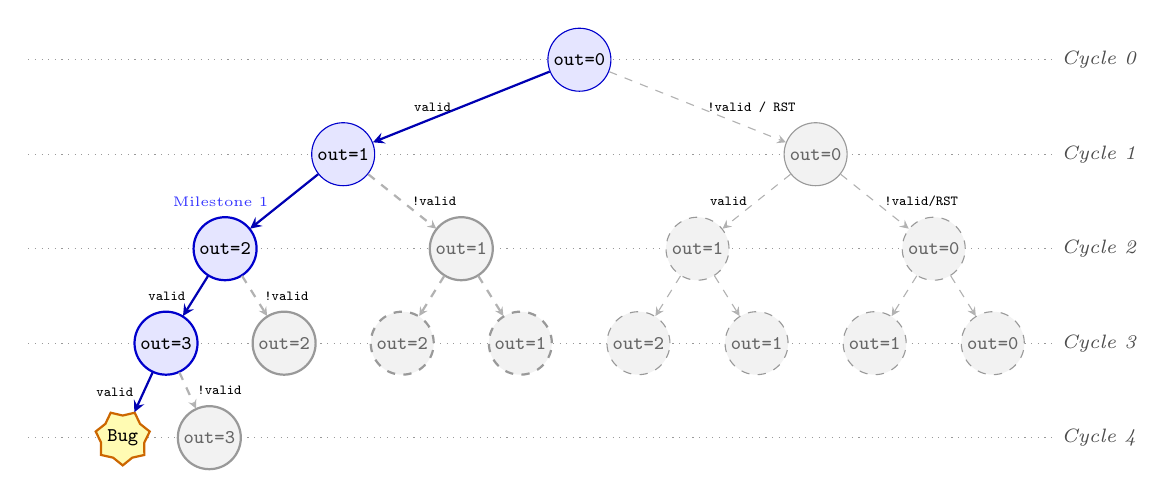
\begin{tikzpicture}[
        >=stealth,
        font=\sffamily\scriptsize,
        level distance=1.2cm,
        % 精准分配每一层的子节点间距，严格防止重叠
        level 1/.style={sibling distance=6.0cm},
        level 2/.style={sibling distance=3.0cm},
        level 3/.style={sibling distance=1.5cm},
        level 4/.style={sibling distance=1.1cm},
        % 节点样式定义
        milestone/.style={draw=blue!80!black, fill=blue!10, circle, minimum size=8mm, inner sep=1pt, font=\bfseries\scriptsize},
        wasted/.style={draw=black!40, fill=gray!10, circle, minimum size=8mm, inner sep=1pt, text=black!60},
        target/.style={draw=orange!80!black, fill=yellow!30, star, star points=7, star point ratio=0.8, inner sep=1.5pt},
        % 连线样式定义
        goodpath/.style={->, thick, draw=blue!70!black},
        badpath/.style={->, draw=black!30, dashed},
        % 标签样式
        cyclelabel/.style={font=\itshape\scriptsize, text=black!70, anchor=west}
    ]

    % 定义树的结构
    \node[milestone] (root) {\texttt{out=0}}
        child {
            node[milestone] (c1_good) {\texttt{out=1}}
            child {
                node[milestone] (c2_good) {\texttt{out=2}}
                child {
                    node[milestone] (c3_good) {\texttt{out=3}}
                    child {
                        node[target] (bug) {\texttt{Bug}}
                        edge from parent[goodpath] node[left, font=\tiny] {\texttt{valid}}
                    }
                    child {
                        node[wasted] (c4_bad) {\texttt{out=3}}
                        edge from parent[badpath] node[right, font=\tiny] {\texttt{!valid}}
                    }
                    edge from parent[goodpath] node[left, font=\tiny] {\texttt{valid}}
                }
                child {
                    node[wasted] (c3_bad1) {\texttt{out=2}}
                    edge from parent[badpath] node[right, font=\tiny] {\texttt{!valid}}
                }
                edge from parent[goodpath] node[left=2pt, font=\tiny, text=blue!80] {Milestone 1}
            }
            child {
                node[wasted] (c2_bad1) {\texttt{out=1}}
                child {
                    node[wasted] (c3_bad2) {\texttt{out=2}}
                    edge from parent[badpath]
                }
                child {
                    node[wasted] (c3_bad3) {\texttt{out=1}}
                    edge from parent[badpath]
                }
                edge from parent[badpath] node[right, font=\tiny] {\texttt{!valid}}
            }
            edge from parent[goodpath] node[left, font=\tiny] {\texttt{valid}}
        }
        child {
            node[wasted] (c1_bad) {\texttt{out=0}}
            child {
                node[wasted] (c2_bad2) {\texttt{out=1}}
                child {
                    node[wasted] (c3_bad4) {\texttt{out=2}}
                    edge from parent[badpath]
                }
                child {
                    node[wasted] (c3_bad5) {\texttt{out=1}}
                    edge from parent[badpath]
                }
                edge from parent[badpath] node[left, font=\tiny] {\texttt{valid}}
            }
            child {
                node[wasted] (c2_bad3) {\texttt{out=0}}
                child {
                    node[wasted] (c3_bad6) {\texttt{out=1}}
                    edge from parent[badpath]
                }
                child {
                    node[wasted] (c3_bad7) {\texttt{out=0}}
                    edge from parent[badpath]
                }
                edge from parent[badpath] node[right, font=\tiny] {\texttt{!valid\\/RST}}
            }
            edge from parent[badpath] node[right, font=\tiny] {\texttt{!valid / RST}}
        };

    % 添加周期标签和横向虚线背景（同步调整了线的宽度以适应新树宽）
    \begin{pgfonlayer}{background}
        \draw[dotted, draw=black!40] (-7.0, 0) -- (6.0, 0) node[cyclelabel] {Cycle 0};
        \draw[dotted, draw=black!40] (-7.0, -1.2) -- (6.0, -1.2) node[cyclelabel] {Cycle 1};
        \draw[dotted, draw=black!40] (-7.0, -2.4) -- (6.0, -2.4) node[cyclelabel] {Cycle 2};
        \draw[dotted, draw=black!40] (-7.0, -3.6) -- (6.0, -3.6) node[cyclelabel] {Cycle 3};
        \draw[dotted, draw=black!40] (-7.0, -4.8) -- (6.0, -4.8) node[cyclelabel] {Cycle 4};
    \end{pgfonlayer}

    \end{tikzpicture}%
    }
    \caption{Symbolic execution tree for the accumulator (Listing \ref{lst:toy_acc}). A standard BFS blindly expands all semantically legal branches (gray nodes), leading to temporal explosion. MileSE leverages intermediate milestones (e.g., \texttt{out==1}, \texttt{out==2}) to strictly prioritize the single path (blue nodes) leading to the assertion violation.}
    \label{fig:sym_tree}
\end{figure}

To illustrate why multi-cycle search is challenging, how milestones help, and what can go wrong, consider the accumulator in Fig.~\ref{fig:verilog-fig} and its corresponding symbolic execution tree in Fig.~\ref{fig:sym_tree}.

%\textbf{Temporal Path Explosion.} 
The assertion violation requires the counter to strictly exceed 3, which demands at least four clock cycles where \texttt{RST} is low and \texttt{valid} is high. As illustrated by the exponentially expanding gray nodes in Fig.~\ref{fig:sym_tree}, a blind symbolic executor utilizing Breadth-First Search (BFS) will fork at every cycle on the \texttt{RST} and \texttt{valid} branches. It wastes massive computational resources exploring semantically legal alternatives---such as continuously asserting reset (\texttt{out <= 0}) or stalling the counter (\texttt{valid == 0})---that never move toward the vulnerable state. 

%\textbf{The Power of Milestones.} 
For this example, useful progress is easy to describe: \texttt{out == 1} $\rightarrow$ \texttt{out == 2} $\rightarrow$ \texttt{out == 3}. As highlighted by the targeted blue path in Fig.~\ref{fig:sym_tree}, if an LLM provides these intermediate conditions as milestones, the engine can prioritize states that satisfy them. Crucially, these milestones provide only a \textit{weak notion of temporal progress}; they are not proof obligations. Instead of permanently injecting them into the path condition, the engine checks whether the current path satisfies the next milestone. If so, the state receives a better priority score and is explored earlier. This transforms a computationally expensive, undirected $2^N$ exploration into a highly targeted progression toward the bug, making the search highly directed without altering the strict formal semantics of the underlying executor.

%\textbf{LLM Hallucinations and Search Stalls.} 
However, naive milestone guidance is inherently unreliable. Since LLMs are probabilistic, they frequently generate flawed milestones. For instance, an LLM might hallucinate an incorrect signal name (e.g., \texttt{rst\_n == 0} instead of \texttt{RST}), propose a physically impossible state transition (e.g., \texttt{out} jumping directly from 0 to 2 in a single cycle), or suggest a condition mathematically inconsistent with the current path constraint. If the formal engine rigidly enforces these flawed milestones, the SMT solver will return UNSAT, causing the search to hit a dead end and fail to find the bug. 

These failure modes fundamentally shape the design of MileSE: the system must leverage the heuristic power of LLM milestones while systematically tolerating their inaccuracies to preserve formal soundness.

\section{MileSE System Architecture}
\label{sec:architecture}

% 请确保在导言区（\begin{document}之前）包含以下宏包：
% \usepackage{tikz}
% \usetikzlibrary{shapes.geometric, shapes.symbols, positioning, fit, backgrounds, arrows.meta}
% 请确保在导言区包含以下宏包：
% \usepackage{tikz}
% \usetikzlibrary{shapes.geometric, shapes.symbols, positioning, fit, backgrounds, arrows.meta}

\begin{figure}[t]
    \centering
    % 使用 \linewidth 完美适配单栏宽度
    \resizebox{\linewidth}{!}{%
    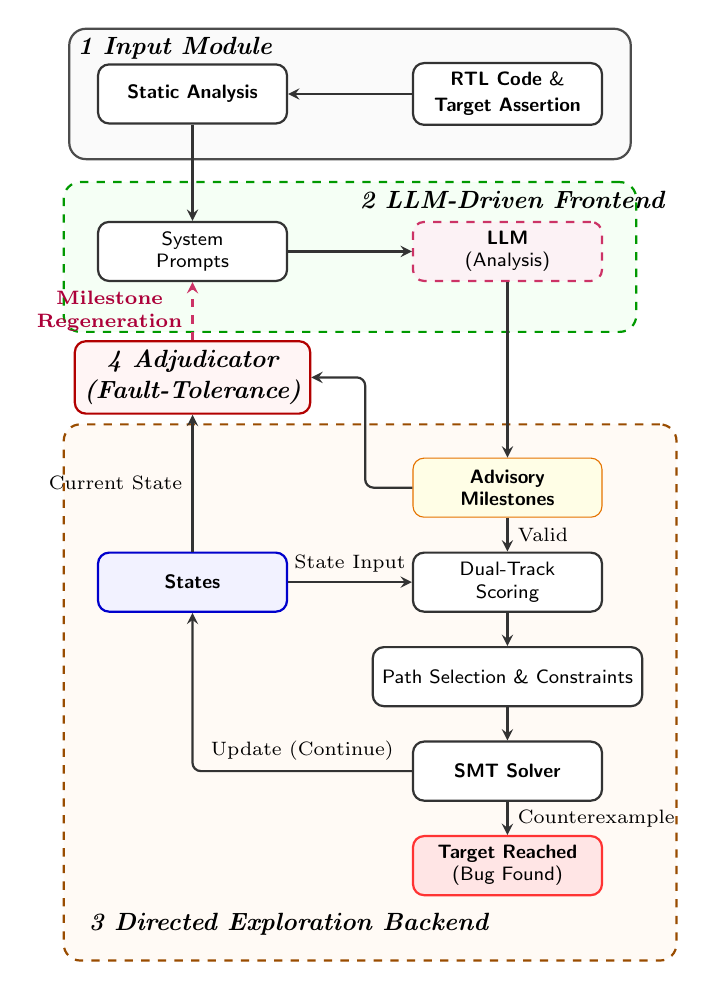
\begin{tikzpicture}[
        font=\sffamily\scriptsize,
        >=stealth,
        % 定义强迫症级别的极简与统一风格
        static_bg/.style={draw=black!70, fill=gray!4, thick, rounded corners=6pt},
        % 全局组件极限瘦身 (高0.75cm, 宽2.4cm)，让内部留白更通透
        inner_box/.style={draw=black!80, fill=white, thick, rounded corners=4pt, minimum height=0.75cm, minimum width=2.4cm, align=center},
        llm_node/.style={draw=black!80, fill=white, thick, rounded corners=4pt, minimum height=0.75cm, minimum width=2.4cm, align=center},
        ms_node/.style={draw=orange!90!black, fill=yellow!10, rounded corners=4pt, minimum height=0.75cm, minimum width=2.4cm, align=center},
        state_node/.style={draw=blue!80!black, fill=blue!5, thick, rounded corners=4pt, minimum height=0.75cm, minimum width=2.4cm, align=center},
        adj_node/.style={draw=red!70!black, fill=red!4, thick, rounded corners=4pt, minimum height=0.75cm, minimum width=2.4cm, align=center},
        score_node/.style={draw=black!80, fill=white, thick, rounded corners=4pt, minimum height=0.75cm, minimum width=2.4cm, align=center},
        smt_node/.style={draw=black!80, fill=white, thick, rounded corners=4pt, minimum height=0.75cm, minimum width=2.4cm, align=center},
        target_node/.style={draw=red!80, fill=red!10, thick, rounded corners=4pt, minimum height=0.75cm, minimum width=2.4cm, align=center},
        arrow/.style={->, thick, draw=black!80, rounded corners=3pt},
        feedback/.style={->, thick, dashed, draw=purple!80, rounded corners=3pt}
    ]

    % 背景层声明
    \pgfdeclarelayer{background}
    \pgfsetlayers{background,main}

    % ==========================================
    % 1. 完美的 2列网格化坐标系 (X = -2.0, X = 2.0)
    % ==========================================
    
    % --- Level 0: 静态输入层 (Y=10.0) 整体上移防重叠 ---
    \node[inner_box] (static_ana) at (-2.0, 10.0) {\textbf{Static Analysis}};
    \node[inner_box] (inputs) at (2.0, 10.0) {\textbf{RTL Code} \&\\[0.05cm]\textbf{Target Assertion}};
    
    \begin{pgfonlayer}{background}
        \node[static_bg, fit=(static_ana) (inputs), inner xsep=10pt, inner ysep=12pt] (static_box) {};
    \end{pgfonlayer}
    \node[anchor=north west, font=\bfseries\small\itshape, text=black] at (static_box.north west) {1 Input Module};

    % --- Level 1: 前端流水线 (Y=8.0) ---
    \node[llm_node] (prompts) at (-2.0, 8.0) {System\\Prompts};
    \node[llm_node, fill=purple!5, draw=purple!80, dashed] (llm) at (2.0, 8.0) {\textbf{LLM}\\(Analysis)};

    % --- Level 1.5: 悬浮的裁决中枢 (Y=6.4) ---
    \node[adj_node, font=\bfseries\small\itshape, text=black] (adjudicator) at (-2.0, 6.4) {\textbf{4} \textbf{Adjudicator}\\(Fault-Tolerance)};

    % --- Level 2: 里程碑 (Y=5.0) ---
    \node[ms_node] (milestones) at (2.0, 5.0) {\textbf{Advisory}\\\textbf{Milestones}};

    % --- Level 3: 状态与评分绝对平行 (Y=3.8) ---
    \node[state_node] (states) at (-2.0, 3.8) {\textbf{States}};
    \node[score_node] (scoring) at (2.0, 3.8) {Dual-Track\\Scoring};

    % --- Level 4 & 5 & 6: 紧凑的执行流水线 ---
    \node[score_node] (path_sel) at (2.0, 2.6) { Path Selection \& Constraints};
    \node[smt_node] (smt) at (2.0, 1.4) {\textbf{SMT Solver}};
    \node[target_node] (target) at (2.0, 0.2) {\textbf{Target Reached}\\(Bug Found)};

    % 隐形锚点撑开底部，给大框的 Label 留出完美安全区
    \node (dummy_bottom) at (0, -0.6) {}; 

    % ==========================================
    % 2. 数据流布线 (神仙级正交，绝对零交叉)
    % ==========================================
    
    % --- Input Module 内部数据流 ---
    \draw[arrow] (inputs.west) -- (static_ana.east);

    % --- 静态分析向下注入前端 ---
    \draw[arrow] (static_ana.south) -- (prompts.north);

    % --- 前端内部交互 ---
    \draw[arrow] (prompts.east) -- (llm.west);
    
    % --- 中轴主流水线下降 ---
    \draw[arrow] (llm.south) -- (milestones.north);
    \draw[arrow] (milestones.south) -- node[right, font=\scriptsize] {Valid} (scoring.north);
    \draw[arrow] (scoring.south) -- (path_sel.north);
    \draw[arrow] (path_sel.south) -- (smt.north);

    % --- SMT 引擎的物理双分支 ---
    % 1. 找到反例 (向下直达终点)
    \draw[arrow] (smt.south) -- node[right, font=\scriptsize] {Counterexample} (target.north);
    
    % 2. 未找到反例 (逆时针回传更新状态)
    \draw[arrow] (smt.west) -| node[pos=0.25, above, font=\scriptsize] {Update (Continue)} (states.south);

    % --- 状态向右交互 ---
    \draw[arrow] (states.east) -- node[above, font=\scriptsize] {State Input} (scoring.west);

    % --- 裁决器 (中场核心) 星型网络 ---
    % 1. States 向上直达 Adjudicator
    \draw[arrow] (states.north) -- node[left, font=\scriptsize] {Current State} (adjudicator.south);
    
    % 2. Milestones 向左折叠进入 Adjudicator
    \draw[arrow] (milestones.west) -- ++(-0.6, 0) |- (adjudicator.east);

    % 3. 裁决失败向上反馈
    \draw[feedback] (adjudicator.north) -- node[left, font=\scriptsize\bfseries, text=purple!90!black, align=center] {Milestone\\Regeneration} (prompts.south);

    % ==========================================
    % 3. 绘制带标题的智能背景虚线框
    % ==========================================
    \begin{pgfonlayer}{background}
        % Frontend 背景框 (单独放大 inner ysep 撑起头部空间)
        \node[fill=green!4, draw=green!60!black, thick, dashed, rounded corners=6pt, 
              fit=(prompts) (llm), inner xsep=12pt, inner ysep=16pt, yshift=-2pt] (frontend_box) {};
        % 标签移至左上角，绝对不遮挡内部组件
        \node[anchor=north west, font=\bfseries\small\itshape, text=black] at (frontend_box.north) {2 LLM-Driven Frontend};
        
        % Backend 背景框
        \node[fill=orange!4, draw=orange!60!black, thick, dashed, rounded corners=6pt, 
              fit=(milestones) (scoring) (path_sel) (smt) (target) (states) (dummy_bottom), inner xsep=12pt, inner ysep=10pt, yshift=2pt] (backend_box) {};
              
        \node[anchor=south west, font=\bfseries\small\itshape, text=black, xshift=6pt, yshift=6pt] at (backend_box.south west) {3 Directed Exploration Backend};
    \end{pgfonlayer}

    \end{tikzpicture}%
    }
    \caption{Overview of the MileSE Framework. (1) Input Module containing RTL code and target assertion undergoes static analysis before being fed into the (2) LLM-driven frontend. Inside the (3) Directed Exploration Backend, generated milestones guide the dual-track scoring and SMT solver. The solver either successfully extracts a counterexample or iteratively updates execution states to continue exploration. In the gap between frontend and backend, the (4) Adjudicator monitors milestone reachability and identifies invalid targets based on current states. Flawed guidance directly triggers a milestone regeneration loop.}
    \label{fig:overview}
\end{figure}


\subsection{Architecture Overview}
The architecture of MileSE, as illustrated in Fig. \ref{fig:overview}, separates the verification process into three functional modules: an \textbf{Input Module} for preprocessing the RTL and target assertions, an \textbf{LLM-Driven Frontend} to generate strategic milestones, a \textbf{Directed Exploration Backend} to execute the milestone-guided path exploration and an \textbf{Adjudicator} to enforce fault-tolerant for flawed milestones. % todo

The verification begins with the Input Module, which performs static analysis on the RTL code and target assertions to extract structural signal dependencies and control flow constraints which are then injected into a pre-defined prompt template alongside the original RTL and assertions. This combined context is sent to the LLM, to generate a sequence of milestones formatted as JSON.

These milestones are then consumed by the Directed Exploration Backend. Within this backend, a \textbf{dual-track scoring mechanism} evaluates candidate paths and directs the exploration to prioritize the branches that are most likely to trigger the bug. To ensure the system get out of the wrong path explorations guided by a flawed milestone, the \textbf{Adjudicator} operates concurrently with a fault-tolerance strategy. During execution, it utilizes a \textbf{sliding-window lookahead} to bypass local temporal mismatches, and a \textbf{timeout-driven regeneration loop} to query the LLM for new milestones if the global exploration stalls. Finally, an \textbf{eager target evaluation} continuously checks the target assertion condition at every cycle, ensuring the bug is caught the moment it becomes reachable, regardless of the whether all milestones are reached.

\subsection{Input Preprocessing and LLM-Driven Planning}
Before the path exploration begins, MileSE initializes the verification task through two sequential modules: a deterministic \textbf{Input Module} for static analysis, followed by an \textbf{LLM-Driven Frontend} for milestone generation.

\subsubsection{RTL Parsing and Static Analysis}
The framework leverages a PySlang frontend to parse the RTL source code, extract its Abstract Syntax Tree (AST), construct procedural control-flow graphs (CFGs), and record combinational dependencies. As an orthogonal optimization, MileSE performs Cone-of-Influence (COI) pruning. Using the target assertion expressions and internal state-update signals, the engine statically removes hardware logic that cannot affect the property, significantly reducing the amount of RTL the execution engine has to carry.

\subsubsection{Prompt Engineering and Milestone Generation}
To ensure the LLM's output is machine-readable and to minimize baseline hallucinations before the dynamic search, MileSE employs a highly structured prompt engineering pipeline rather than feeding raw RTL code. 


The prompt context is constructed with three base inputs: (1) the \textit{Target Assertion}, which specifies the exact property or condition to be verified; (2) the \textit{CFGs(Control Flow Graphs)}, which provide the model with explicit structural branching logic; and (3) the \textit{Original RTL code}, which supplies the underlying hardware description. Furthermore, if the Cone-of-Influence (COI) technique is applied, the system refines these inputs to yield the COI-pruned RTL code and a correspondingly reduced CFG. This pruning step drastically cuts down the token overhead by filtering out irrelevant hardware logic, ensuring the critical design context fits well within the LLM's context window, and reduce the total paths to be explored.

To prevent formatting hallucinations and enable automated parsing by the Directed Exploration Backend, the LLM is strictly instructed to output the milestones matching a standardized JSON template. As shown in Listing \ref{lst:json_template}, each milestone must explicitly declare its expected clock cycle budget (\texttt{cycle\_bound}) and a mathematically verifiable RTL expression (\texttt{condition}). 

Through this template-driven approach, MileSE breaks down a complex verification target into a series of step-by-step RTL sub-goals. This provides the backend engine with a clear roadmap, telling it exactly which RTL conditions to satisfy and the clock cycle budget for each step.

\begin{lstlisting}[language=json, aboveskip=1.5em, belowskip=1em, caption={Standardized JSON template for LLM milestone generation.}, label={lst:json_template}, basicstyle=\ttfamily\scriptsize, frame=single, numbers=left, xleftmargin=2em]
{
  "milestones": [
    {
      "step": 1,
      "intent": "Release system reset and wait for initialization",
      "cycle_bound": 2,
      "condition": "RST == 1'b0"
    },
    {
      "step": 2,
      "intent": "Trigger the valid signal to start accumulation",
      "cycle_bound": 5,
      "condition": "valid == 1'b1 && out == 32'd1"
    }
  ]
}
\end{lstlisting}

\subsection{Dual-Track Directed Search}
To prevent the execution from degenerating into undirected Breadth-First Search (BFS) during multi-cycle intervals between milestones, MileSE introduces a Dual-Track Scoring strategy. This mechanism practically combines the LLM's high-level milestones with the engine's cycle-level structural feedback. Each symbolic state $n$ in the priority queue is ranked by a unified scoring function $f(n)$:
\begin{equation}
    f(n) = \alpha \cdot R(n) + C(n) + \min(D(n), D_{\max})
\end{equation}
where a lower score indicates a higher execution priority.

\textbf{Global Milestone Track.} $R(n)$ counts the number of milestones remaining, while $C(n)$ tracks the elapsed clock cycles. A dominant weight $\alpha$ ensures the engine's top priority is to advance through the milestone sequence. When multiple states share the exact same milestone progress, the engine simply compares their $C(n)$ values, naturally selecting the path that arrived there using fewer clock cycles.

\textbf{Local Gradient Track.} When milestone progress stalls over multiple cycles, the distance metric $D(n)$ takes over to guide the search. Instead of invoking a heavy SMT solver, MileSE calculates this distance directly based on the generated CFGs. By measuring the structural gap between the current state's position and the target condition in the CFG, $D(n)$ provides a lightweight local gradient, steering the execution step-by-step toward the next milestone.

\textbf{Preferred-Path Execution.} To maximize execution speed, MileSE adopts a strict branching strategy. When the engine evaluates a conditional branch, it does not explore all possible paths simultaneously. Instead, it exclusively executes the single "preferred path" with the best $D(n)$ score. Any other valid sibling branches are paused, saved as checkpoints, and deferred to a pending state pool (represented as the States node in Fig. \ref{fig:overview}). This ensures that expensive SMT resources are focused entirely on the most direct path to the milestone, rather than wasting time on irrelevant branches.


\subsection{Fault-Tolerant Adjudication}
%A naive integration of LLMs often causes engines to stall when milestones contain hallucinated signals or unreachable temporal states. To handle this, the \textbf{Adjudicator} in MileSE evaluates all milestones using non-intrusive speculative queries (e.g., \texttt{push} and \texttt{pop}) to prevent constraint pollution. Building upon this safe baseline, the Adjudicator ensures continuous execution and verification accuracy through three core fault-tolerant mechanisms. Specifically, it achieves \textbf{local recovery} via a sliding-window lookahead, executes \textbf{global recovery} through timeout-driven dynamic re-planning, and provides \textbf{fail-safe bug detection} via eager target evaluation.

A naive integration of LLMs often causes engines to stall when milestones contain hallucinated signals or unreachable temporal states. To handle this, the Adjudicator ensures continuous execution and verification accuracy through three core fault-tolerant mechanisms. Specifically, it achieves \textbf{local recovery} via a sliding-window lookahead, executes \textbf{global recovery} through timeout-driven dynamic re-planning, and enables \textbf{immediate bug capture} via eager target evaluation.

\subsubsection{Sliding-Window Lookahead}
To counter local temporal mismatches (e.g., the hardware transitions directly from state $0$ to $2$, bypassing milestone $1$), MileSE employs a Sliding-Window Lookahead. If the immediate milestone $M_{i}$ remains unresolvable, the engine non-blockingly evaluates the next target $M_{i+1}$. If this future milestone evaluates to \texttt{SAT}, the engine automatically shifts its focus and drops the bypassed intermediate milestones, avoiding getting stuck on the unreachable states.

\subsubsection{Timeout-Driven Dynamic Re-Planning}
When a milestone sequence fundamentally diverges from the reachable state space, local lookahead is insufficient. MileSE uses the milestone's \texttt{cycle\_bound} metric $k$ as a flexible timeout threshold. By introducing a constant tolerance margin $\Delta$, if a state fails to make progress after $k + \Delta$ cycles, the Adjudicator determines that the current sequence is unreachable. Instead of getting stuck indefinitely, it leverages the state-feedback mechanism (labeled \textit{Milestone Regeneration} in Fig. \ref{fig:overview}). The Adjudicator halts the stalled branch, extracts the verifiable state conditions from the pending state pool, and feeds them back to the LLM to dynamically generate a new, locally reachable milestone sequence that is more likely to be reachable.

\subsubsection{Eager Target Evaluation}
While intermediate milestones guide the heuristic exploration, they cannot be trusted to validate the final target. To ensure no actual bugs are ever missed, MileSE implements Eager Target Evaluation. Throughout the execution, the engine continuously monitors the global target assertion. If the target condition is satisfied, MileSE instantly terminates the exploration and generate counterexample trace. This guarantees that the vulnerability is captured the moment it becomes reachable, completely independent of the LLM's milestones.

\section{Experimental Evaluation}
\label{sec:evaluation}

Our experimental evaluation is structured around two primary dimensions:

\textbf{1: Mitigation of Path Explosion.} Demonstrating that milestone-guided scheduling effectively mitigates temporal path explosion on deep RTL properties while maintaining strict execution reliability.

\textbf{2: Ablation of Fault-Tolerance Mechanisms.} Quantifying the individual performance contributions of the sliding-window lookahead and eager target evaluation to the overall system gains.

\subsection{Implementation and Experimental Setup}
The experiments are conducted on a computer with AMD Ryzen 9 9950x3d CPU, 96GB RAM and the operating system is Ubuntu 24.04.  We implemented MileSE as a custom Python-based symbolic execution engine. The frontend leverages \textbf{PySlang}\cite{pyslang} for rigorous SystemVerilog parsing,  and cycle-accurate AST generation. Formal checking is powered by the \textbf{Z3 SMT solver}\cite{z3}. The engine dynamically constructs CFGs, applies COI pruning on the AST prior to Z3 query formulation, and integrates the dual-track priority queue and fault-tolerance mechanisms described in Section~\ref{sec:architecture}. %LLM milestone generation is handled via API calls to an instruction-tuned model. 


\subsection{Benchmarks and Baselines}
\label{subsec:setup}

We evaluate on four representative multi-cycle RTL security benchmarks \cite{rogers2024securityproperties}:
\begin{itemize}
    \item \textbf{HACK@DAC\,18/19/21}: SoC-level security competition benchmarks containing hardware Trojan and privilege-escalation bugs requiring multi-cycle trigger sequences across complex bus fabrics and debug interfaces. We evaluate a total of 19, 11, and 17 distinct properties from these three versions, respectively.
    \item \textbf{OR1200}: An open-source RISC processor core instrumented with 71 sequential assertion properties covering pipeline control, exception handling, and memory access ordering.
\end{itemize}

We compare four configurations that isolate the contribution of each component:
\begin{itemize}
    \item \textbf{Baseline}: Milestone-directed search with \emph{neither} sliding-window lookahead nor eager target evaluation enabled.
    \item \textbf{+Eager}: Adds eager target evaluation only (\texttt{--no-sliding} flag disabled).
    \item \textbf{+Sliding}: Adds sliding-window lookahead only (\texttt{--no-eager} flag disabled).
    \item \textbf{Full}: Both mechanisms enabled (the complete MileSE system).
\end{itemize}

All four configurations share identical LLM-generated milestones, the same COI pruning, and the same Z3 backend, so differences in outcomes are attributable solely to the fault-tolerance mechanisms under study.

\subsection{Overall Verification Performance}
\label{subsec:eval_overall}

% TODO: Insert the overall performance evaluation here.
% This section should compare the Full MileSE system against EXTERNAL state-of-the-art baselines 
% (e.g., standard symbolic execution engines, classical bounded model checking tools) to demonstrate overall superiority.


\subsection{Ablation Study: Fault-Tolerance Mechanisms}
\label{subsec:eval_ablation}

To answer our second research objective, Table~\ref{tab:main_results} summarizes violations found, timeouts, average runtime on non-timeout runs, and average SMT queries per property across all benchmarks and internal configurations. 

\begin{table}[htbp]
    \centering
    \caption{Verification results across benchmarks and ablation conditions.
    \#Viol = properties with confirmed violation;
    T.O. = timeouts;
    Avg-$t$ = average total runtime on non-timeout runs (seconds);
    Avg-SMT = average SMT queries per non-timeout property.}
    \label{tab:main_results}
    % 使用 \resizebox 强制将其约束在单栏宽度内
    \resizebox{\columnwidth}{!}{%
    \begin{tabular}{@{}llrrrr@{}}
        \toprule
        \textbf{Benchmark} & \textbf{Config} & \textbf{\#Viol} & \textbf{T.O.} & \textbf{Avg-$t$ (s)} & \textbf{Avg-SMT} \\
        \midrule
        \multirow{4}{*}{HACK@DAC\,18 (19)}
            & Baseline  & 12 & 3 & 29.6 & 3927 \\
            & +Eager    & 14 & 3 & 23.4 &  645 \\
            & +Sliding  & 12 & 3 & 29.5 & 3287 \\
        \cmidrule{2-6}
            & \textbf{Full} & \textbf{14} & 3 & \textbf{23.9} & \textbf{674} \\
        \midrule
        \multirow{4}{*}{HACK@DAC\,19 (11)}
            & Baseline  & 11 & 0 & 181.9 & 2535 \\
            & +Eager    & 10 & 1 &  47.3 &  760 \\
            & +Sliding  & 11 & 0 & 184.4 & 2484 \\
        \cmidrule{2-6}
            & \textbf{Full} & \textbf{10} & 1 & \textbf{47.3} & \textbf{760} \\
        \midrule
        \multirow{4}{*}{HACK@DAC\,21 (17)}
            & Baseline  & 15 & 2 & 100.5 & 10526 \\
            & +Eager    & 15 & 2 &  83.8 &  6536 \\
            & +Sliding  & 15 & 2 & 101.1 & 12185 \\
        \cmidrule{2-6}
            & \textbf{Full} & \textbf{15} & 2 & \textbf{80.3} & \textbf{5978} \\
        \midrule
        \multirow{4}{*}{OR1200 (71)}
            & Baseline  &  69 & 2 &  5.1 &  893 \\
            & +Eager    & 70 & 1 & 12.6 & 3658 \\
            & +Sliding  &  70 & 1 &  5.2 &  891 \\
        \cmidrule{2-6}
            & \textbf{Full} & \textbf{9} & 62 & \textbf{9.1} & \textbf{2287} \\
        \bottomrule
    \end{tabular}%
    }
\end{table}

\subsubsection{Performance by Benchmark}

\textbf{HACK@DAC Results.}
Across the three SoC benchmarks, MileSE Full consistently finds the most violations or matches the best configuration. On HACK@DAC\,18, Full and +Eager both detect 14 violations against 12 for the two sliding-only and baseline runs. The key differentiator is solver overhead: Full reduces average SMT queries from 3,927 (Baseline) to 674—a \textbf{5.8$\times$ reduction}—while +Eager alone achieves 645 queries, confirming that eager target evaluation is the primary driver of solver efficiency on this benchmark. On HACK@DAC\,21, Full achieves the lowest average runtime (80.3\,s vs.\ 100.5\,s for Baseline) and the fewest average SMT queries (5,978 vs.\ 10,526), a \textbf{1.8$\times$ SMT reduction} with the same violation count.

HACK@DAC\,19 exhibits a notable asymmetry: +Sliding and Baseline both find 11 violations with zero timeouts, whereas Full and +Eager find only 10 violations but time out once. Inspection reveals that property \texttt{HACKDAC\_p5} is detected only in the sliding-window configurations. In this case, the eager-target-evaluation check fires prematurely on a spurious near-miss path, consuming the time budget before the correct path is explored. This is an identified limitation of the current suppression threshold and motivates future adaptive tuning of the eager-check window.

\textbf{OR1200 Results.}
The processor benchmark is the most challenging: the baseline finds only 2 violations (69 timeouts out of 71 properties). Adding eager target evaluation (+Eager) jumps the detection count to 11 violations and reduces timeouts to 60. The Full configuration finds 9 violations (62 timeouts), slightly fewer than +Eager alone. The difference arises because the sliding-window component occasionally skips a milestone that was feasible, redirecting the search away from some bugs that the eager-only path would find. Despite this trade-off, Full still represents a \textbf{4.5$\times$} improvement over Baseline in bugs found. The overall high timeout rate on OR1200 reflects the depth of its sequential properties (10 cycles) against a 300\,s budget, and is consistent with prior work on processor symbolic execution.

\subsubsection{Isolated Component Contributions}

\textbf{Eager Target Evaluation.}
Comparing +Eager against Baseline isolates the impact of the eager final-milestone pre-check. On HACK@DAC\,18, +Eager adds 2 violations and cuts average SMT queries by $6.1\times$. On OR1200, +Eager is the dominant mechanism, recovering 9 additional violations that Baseline misses entirely. The mechanism is most impactful when the final milestone is satisfiable earlier than the nominal expected cycle, a common pattern in security bugs where a single-cycle race condition invalidates the milestone schedule.

\textbf{Sliding-Window Lookahead.}
Comparing +Sliding against Baseline isolates the lookahead contribution. On the HACK@DAC benchmarks, +Sliding has negligible effect on violation count but offers moderate SMT reduction (e.g., 3,287 vs.\ 3,927 on HACK@DAC\,18), showing that the window primarily suppresses redundant solver calls on hallucinated milestones. On OR1200, +Sliding provides no additional violations over Baseline. The lookahead window of size 1 is designed for conservative milestone skipping and is most beneficial when LLM-generated intermediate milestones are temporally misaligned rather than globally unreachable.

\textbf{Combined Effect.}
When both mechanisms are active (Full), the interaction is largely additive on the HACK@DAC benchmarks, achieving the best runtime and SMT efficiency simultaneously. On OR1200, the mechanisms partially interfere—eager evaluation opens new paths that the sliding-window skip subsequently misdirects—but Full still dominates Baseline by a wide margin. These results suggest that eager target evaluation should be prioritized when maximizing bug-finding rate, while sliding-window lookahead is the safer default for reducing solver overhead in LLM-hallucination-heavy scenarios.

\section{Related Work}
\label{sec:related}
% ... [Rest of your Related Work text] ...

\section{Conclusion}
\label{sec:conclusion}
MileSE addresses the temporal path explosion bottleneck in multi-cycle RTL symbolic execution by combining LLM-generated milestone guidance with two synergistic fault-tolerance mechanisms: sliding-window lookahead and eager target evaluation. Experiments across four hardware security benchmarks (118 properties total) demonstrate that MileSE Full recovers up to $4.5\times$ more bugs than the baseline on the OR1200 processor and reduces SMT solver queries by up to $5.8\times$ on HACK@DAC\,18, while maintaining formal soundness throughout. The ablation study shows that eager target evaluation is the primary driver of bug-finding rate, whereas sliding-window lookahead contributes most to solver overhead reduction in LLM-hallucination-heavy scenarios. Together, these mechanisms allow MileSE to safely prune the multi-cycle state space without injecting false negatives, making it a practical and sound framework for deep sequential RTL verification.

\section*{Acknowledgment}
Acknowledgment text will be finalized in the camera-ready version.

\bibliographystyle{IEEEtran}
\bibliography{ref}

\end{document}
